
%Batteries are important

%Use EM to analyze them

%In particular EELS is good

%Want simulations, use DFT
 
%Want better simulations improve core hole method
\setcitestyle{numbers,open={[},close={]}}

The study of lithium materials has become increasingly relevant in recent years \cite{nitta_li-ion_2015}.  In particular, the field has been driven by the need to develop improved  and more cost effective battery materials \cite{nitta_li-ion_2015}.  This drive has come from increasing demands for electric vehicles and portable electrical devices demanding longer lifetimes and faster charging.  Many aspects of  batteries can be improved as the theoretical limits have not yet been achieved in fundamental areas such as capacity, charge density, and charge/discharge rates. \\


The theoretical limits in the case of lithium ion batteries are especially high, as lithium offers a range of advantages relative to other charge carriers. As the third element on the periodic table, lithium is extremely lightweight, allowing lithium ion batteries to be smaller and lighter without sacrificing lifetime \cite{etacheri_challenges_2011}.  Lithium's small ion size makes it highly mobile, which leads to superior discharge rates  \cite{etacheri_challenges_2011}.   Furthermore, as an alkali earth metal with a single weakly bound valence electron, lithium is highly electropositive.   As a result, lithium ion batteries can achieve higher operating voltages than alternatives such as nickle-cadmium or lead-acid batteries \cite{etacheri_challenges_2011}.  Some of these comparative performance advantages to these alternatives are illustrated in Fig \ref{ragone} \cite{etacheri_challenges_2011}.\\

\begin{figure}
	\centering
	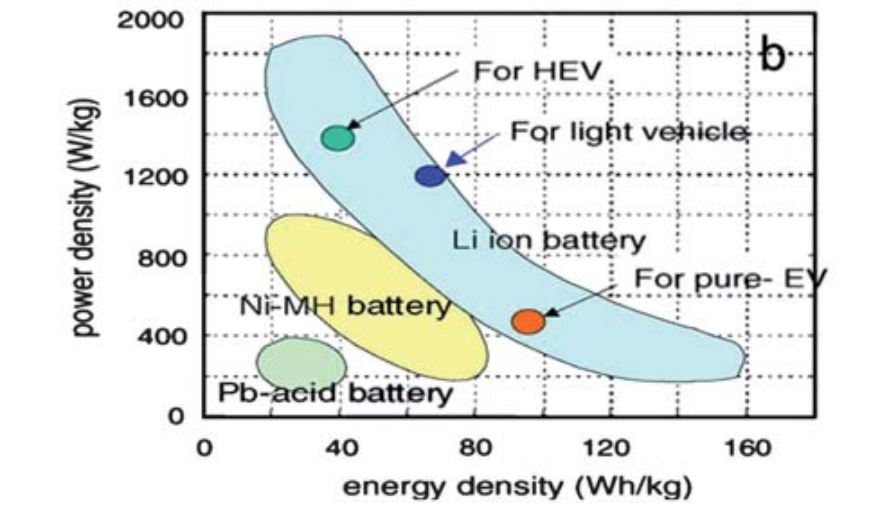
\includegraphics[width=0.5\textwidth]{ragone_plot}
	\caption{Plot illustrating the the power and energy densities achievable by three types of battery, as well as the minimum requirements for various types of electric vehicle, including hybrid electric vehicles (HEV), plug in hybrids (light vehicle). From Etacheri, 2011 \cite{etacheri_challenges_2011}. }
	\label{ragone}
	
\end{figure}
The pursuit of further improving the performance of lithium batteries has shifted analysis of these materials increasingly towards measuring microstructure properties \cite{lu_lithium_2012,arthur_spontaneous_2016, muller_quantification_2018}. Identifying microscale features such as crystal structure, diffusion mechanics, and composition is an essential component of characterizing new battery materials \cite{van_der_ven_first-principles_2001}. These features are being increasingly analyzed through electron microscopy, which offers the high spatial resolution needed to analyze them and is becoming increasing accessibility   \cite{chiu_aqueous_2013,inkson_2_2016, hansen_atomic-resolution_2001}. \\

Lithium materials however, present a range of challenges to electron microscopy.  Battery materials are becoming increasingly intricate and lithium's light weight and ionizable nature make it particularly susceptible to electron beams \cite{kobayashi_quantitative_2017}.  This sensitivity limits analysis largely to low dosage techniques to avoid damaging the samples long enough to acquire results.  One such technique that is targeted for light elements, such as lithium, is electron energy loss spectroscopy (EELS) \cite{Egerton}.  However, even using low dosage techniques,  beam damage remains problematic for lithium materials.  Recent developments such as low voltage EELS are allowing lithium analysis to become more routine \cite{SU_9000}. As these new experimental techniques produce unprecedented results, a degree of theoretical support is required to confirm the methods and explain any irregularities.  
\\

Theoretical support for EELS  comes most predominantly from methods based in density functional theory (DFT). DFT is a first principles method capable of calculating materials properties using only the crystal structure as input.  As in experiment however, lithium's lightweight nature complicates DFT calculations and results have been limited to qualitative findings \cite{mauchamp_ab_2006, mauchamp_local_2008}. Much of the challenge in simulating EELS for lithium lies in the treatment of the electron hole created in excited atoms.  Lithium's few electrons mean that core hole effects will almost always be present in the spectra which current methods in literature lack the subtlety to treat. \\

The goal of this work is to calculate meaningful EELS spectra of lithium materials, in particular, the K edge near edge structure, in the unprecedented context of EELS at 30 keV. This is accomplished be improving the treatment of core electron holes of lithium in DFT simulations. \\

The outline of this thesis is as follows: Chapter \ref{literature_review} presents an overview of EELS, DFT and theoretical EELS calculations.  Chapter \ref{methods} describes the improved method developed in this work, and Chapter \ref{results} applies the method to a number of lithium materials.  Chapter \ref{conclusion} concludes the results and addresses future work.


